\documentclass{bioinfo}

\usepackage{relsize} % for Cpp
\usepackage{xspace} % for Cpp

\newcommand{\odgi}{ODGI}
\newcommand{\cmd}[1]{{\texttt{#1}}}
\newcommand{\cmdbf}[1]{{\textbf{#1}}}
\newcommand{\topic}[1]{{\cmdbf{#1}}:}
\newcommand{\Rplus}{\protect\hspace{-.1em}\protect\raisebox{.35ex}{\smaller{\smaller\textbf{+}}}}
\newcommand{\pp}{\Rplus\Rplus}
\newcommand{\Cpp}{\mbox{C\Rplus\Rplus}\xspace}


\copyrightyear{2021} \pubyear{2021}

\access{Advance Access Publication Date: Day Month Year}
\appnotes{Manuscript Category}

\begin{document}
    \firstpage{1}

    \subtitle{Genome Analysis}

    \title[ODGI: scalable tools for pangenome graphs]{ODGI: scalable tools for pangenome graphs}
    \author[Sample \textit{et~al}.]{
        Andrea Guarracino\,$^{\text{\sfb 1,}*}$,
        Simon Heumos\,$^{\text{\sfb 2}}$,
    % XXXXX,
        Pjotr~Prins\,$^{\text{\sfb 3}}$ and
        Erik~Garrison\,$^{\text{\sfb 3,}*}$
    }
    \address{$^{\text{\sf 1}}$Department, Institution, City, Post Code, Country \\
        $^{\text{\sf 2}}$Department, Institution, City, Post Code, Country \\
        $^{\text{\sf 3}}$Genetics Genomics \& Informatics, UTHSC, Memphis, TN, USA
    }

    \corresp{$^\ast$To whom correspondence should be addressed.}

    \history{Received on XXXXX; revised on XXXXX; accepted on XXXXX}

    \editor{Associate Editor: XXXXXXX}

    \abstract{
        \textbf{Motivation:} Pangenome graphs provide a complete representation of
        genomic information that allows for complex population-sized analysis of genomes
        without introducing reference genome bias.
        %
        \\
        \textbf{Results:} Here we present \odgi\, a novel range of tools that makes use of an efficient
        in-memory representation of DNA graphs structured in the variation graph model. \odgi\ can
        handle hundreds of large genomes while maintaining fast execution runtime and low memory overhead.
        \odgi\ includes tools for detecting complex regions, extracting \textit{loci}, exploratory analysis,
        sorting, removing artifacts, and graphs manipulation and visualisation.
        %
        \\
        \textbf{Availability:} \odgi\ is software written in the \Cpp\ programming language and
        published under the libre MIT license. Source code and user manual can be downloaded from
        \href{https://github.com/pangenome/odgi}{https://github.com/pangenome/odgi}.\\
        %
        \textbf{Contact:}
        \href{andreaguarracino@outlook.com}{andreaguarracino@outlook.com},
        \href{erik.garrison@gmail.com}{erik.garrison@gmail.com}\\
        \\textbf{Supplementary information:} Supplementary data are available at \textit{Bioinformatics} online.}

    \maketitle


    \section{Introduction}

    A pangenome models the full set of genomic elements in a given species or clade~\citep{32453966}. Indeed, these
    data structures encode the mutual relationships between all the genomes represented, in contrast to reference-based
    approaches which relate sequences only to a particular genome, chosen as reference. A class of methods to represent
    pangenomes involves the \textit{sequence graphs}~\citep{2488477}, where similar orthologous regions between genomes
    collapse into a single representative sequence. In \textit{node-labeled} sequence graphs, nodes indicate DNA
    sequences, with edges connecting the nodes that are concatenated in the sequences represented in the graph. A
    \textit{bidirected} sequence graph represents both strands of DNA. On this model, \textit{variation graphs} add the
    concept of \textit{path} to embed linear sequences (e.g., genomes or haplotypes) into the graph~\citep{30125266}.
    Paths provide a stable coordinate system, allowing graph annotations and interoperability between different graphs.

    Thanks to advances in sequencing technologies, new genome assemblies are produced at a high rate. This amount of
    data offers the opportunity to study genomic variation as never before, but it also brings challenges in how to
    represent and manipulate hundreds of genomes at a gigabase scale. Variation graphs compactly represent the full
    genetic variation across a population, but graph-based data structures present computational overheads: in addition
    to the sequences, they must also represent the graph topology. Several genome data structures were developed to
    address these challenges~\citep{33040146}. Memory-efficient representations do not allow dynamic updates to the
    graph, such as adding new genomes or simplifying the graph topology. Furthermore, dynamic updates must perform
    efficiently on the complex graphs generated from whole-genome alignment of vertebrates. Highly repetitive regions,
    such as centromeres, segmental duplications, and acrocentric chromosomes lead to graphs which present paths with
    very high-depth nodes. The node depth is defined as the number of times in which the node is crossed by all the
    paths embedded in the graph. High depth increases the complexity of the operations performed on the paths and the
    nodes they cross.

    To overcome this limitation, we have developed an Optimized Dynamic Genome/Graph Implementation (ODGI). Each tool
    loads graphs into the succinct dynamic HandleGraph model~\citep{33040146} and applies methods based on the
    HandleGraph API. Several algorithms are shared with the VG toolkit (VG)~\citep{30125266}, the state-of-the-art
    toolkit for working with pangenome graphs. However, although similar in scope to VG, \odgi\ importantly differs in
    its design to support highly complex pangenome graphs. The majority of the \odgi\ tools are implemented in an
    index-free manner, avoiding the burning task needed to create an index structure. Indeed, index-constrained
    implementations would require building indexes also for single or little operations on the graphs. Moreover,
    thanks to its efficient path representation, \odgi\ tools can build the internal graph representation (the \odgi\
    format) in parallel, which is one of the major bottlenecks when working with very large and deep variation graphs,
    efficiently scaling up to hundreds of large vertebrate genomes.

    \odgi\ is entirely focused on "first-order" operations on the graph
    (Table~\ref{tab:01}), providing, unlike VG, no method to construct
    graphs from raw sequences, map reads, or call variants. It
    supports interrogation of the graph for basic dimensional
    properties, positional and path-related queries, and visualization
    in one-dimension (1D) and two-dimensions (2D). \odgi\ also supports
    operations on the graph such as subset, subdivide, break, combine,
    normalize, or order its components, nodes, and paths. Most of the
    tools are designed to be applied together, piping the output of
    one tool into the next, thereby preventing the creation of
    intermediate files, and reducing the number of IO operations.

    \section{Methods}

    \odgi\ is designed to build and modify paths in parallel, keeping its representation in memory efficient. It
    applies concepts first introduced in the dynamic version of the Graph BWT~\citep{31406990}, a scalable
    implementation of the graph extension of the positional Burrows-Wheeler transform~\citep{28702075}. Specifically,
    we build a \textit{node-local} model of the graph, where the graph is stored in a vector of node structures.
    The identifier of each node is its offset in this vector plus 1. Each structure contains the sequence of the
    node, its edges in both directions (forward and backward), and a vector of \textit{path steps} that describes
    how the embedded paths walk across the node. Each step records the path identifier and the previous and next
    path steps on the same path. To reduce the encoding, we encode path steps using a local alphabet that maps the
    \textit{N} neighbors of the node into the range \textit{1..N}. To further save space, \textit{node deltas},
    rather than IDs, are stored in this alphabet. The delta between two nodes is defined as their distance in the
    graph vector (i.e., the difference between the node offsets). The path step vector, of length \textit{n}, is
    stored using a dynamic succinct integer vector that requires \textit{O(5nw)} bits, where \textit{w} is
    \textit{\textasciitilde log\textsubscript{2}(N)}. Finally, to allow operating on path steps in parallel, each node
    structure includes a byte-width mutex lock.


    \section{Results}

    \odgi\ has a wide range of commands.

    \topic{odgi build, view \& validate} pangenome graphs are commonly
    represented by a subset of Graphical Fragment Assembly (GFAv1)
    format \citep{GFAv1}; \cmd{odgi build} and \cmd{odgi view} allow
    to convert graphs from GFA to \odgi\ format and vice versa. In the
    variation graph model, paths have to respect the graph's topology:
    this can be verified with \cmd{odgi validate}, to ensure no
    errors in the input or edited graphs.

    \topic{odgi viz, sort, drawn \& layout} by visualizing pangenome
    graphs, we can gain insight into the relationship between
    genomes. \cmd{odgi viz} applies binding and direct rendering to
    a raster image to generate a 1D representation able to scale up to
    gigabase pangenome graphs (Figure~1\vphantom{\ref{fig:1}}).
    However, pangenome graphs may present complex structures to
    visualize: \cmd{odgi sort} finds the best node order to simplify
    1D graph visualization by applying several cutting-edge sorting
    algorithms. \cmd{odgi drawn} extends the visualization in 2D,
    taking in input the layouts built by \cmd{odgi layout}.

    \topic{odgi stats, bin, depth \& degree} users can retrieve metrics describing the graph properties, such as the number of
    nodes, edges, paths, and graph length. \odgi\ also offers more advanced tools for interrogating the graphs.
    \cmd{odgi bin} summarizes the path information into bins of specified size, enabling a summarized view of
    gigabase scale graphs. \cmd{odgi depth} returns the node depth as defined by query criteria, allowing users to
    detect the complex regions in the graph due to sequences with highly identical repeats. Complex motifs can be also
    detected with \cmd{odgi degree}, which returns the node degree as defined by query criteria. High degree nodes
    are the mirror of misassemblies or problems in the pangenome building, making the tool useful for debugging the
    process as well.

    \topic{odgi break, groom, chop \& unchop} \odgi\ allows edit operations on the graphs. Cycles in the graph
    complicate downstream analyses: \cmd{odgi break} removes the cycles, reducing the complexity of the graph topology.
    \cmd{odgi groom} removes spurious inverting links by exploring the graph from the orientation supported by most
    paths. To enable efficient sequence alignment against the graph, long nodes can be divided into shorter nodes
    at a maximum requested size using \cmd{odgi chop}. Partial order alignment, which consists of aligning sequences
    against a directed acyclic graph (DAG), is frequently used in pangenome building pipelines, but the current
    implementations return DAGs with 1-bp long nodes; \cmd{odgi unchop} allows joining nodes that can be merged
    without changing the graph topology, nor the embedded sequences, obtaining an equivalent, but more compact,
    representation of the graph.

    \topic{odgi explode, squeeze \& extract} pangenome graphs can embed multiple chromosomes as separated connected
    components (inter-chromosomal structural variants would join the components into bigger ones).
    \cmd{odgi explode} separates the connected components in different \odgi\ format files, while \cmd{odgi squeeze}
    allows merging multiple graphs into the same \odgi\ format file, preventing node ID collisions. \cmd{odgi extract}
    allows extracting specific subregions of the graph as defined by query criteria, thereby simplifying the downstream
    analyses and reducing the resources to work only with the extracted region.

    \topic{odgi position} in variation graphs the coordinates are provided by the embedded path sequences. Indeed, the node
    IDs are not meant to be stable. \cmd{odgi position} finds, translates, and liftovers graph and path positions between
    different graphs by exploiting their shared path sequences (Figure~2\vphantom{\ref{fig:2}}).

    \begin{figure}
        \begin{minipage}[b]{0.48\textwidth}
            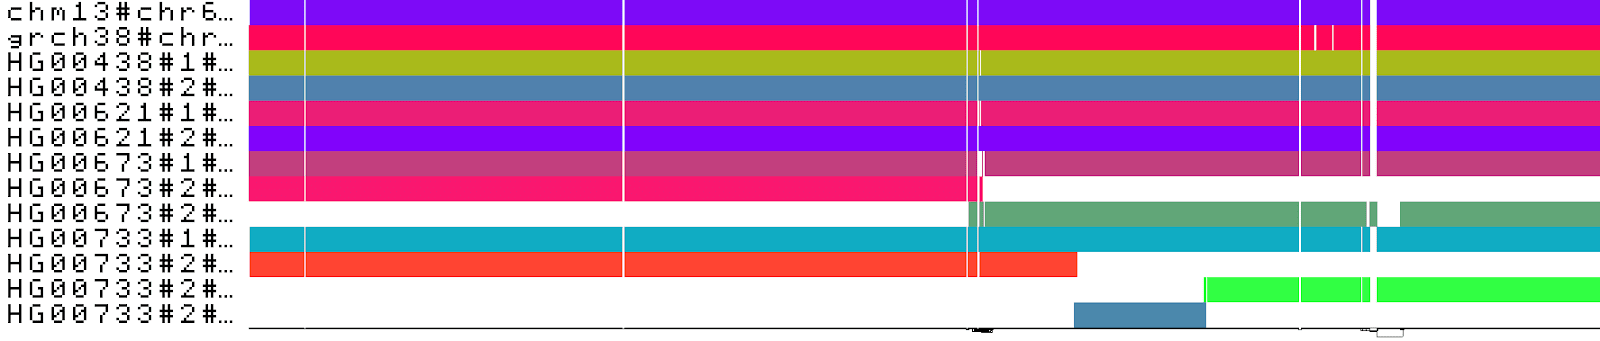
\includegraphics[width=\linewidth]{fig/mhc-align}
            \caption{(a) alignment}
            \label{fig:1}
        \end{minipage}

        \begin{minipage}[b]{0.48\textwidth}
            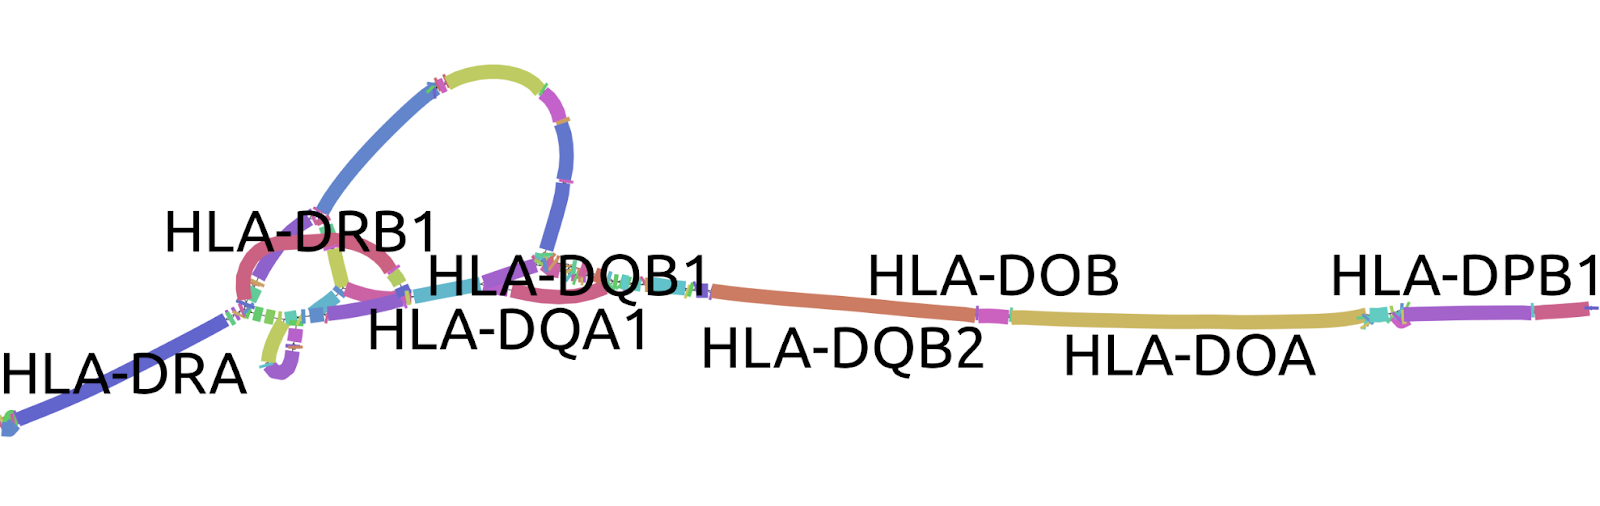
\includegraphics[width=\linewidth]{fig/mhc-pangenome}
            \caption{(b) Visualizing the Major Histocompatibility Complex
                (MHC) \textit{locus} pangenome. A) \cmd{odgi viz} 1D visualization
                of 8 haploid, phased human genome assemblies plus the chm13
                and GRCh38 reference genomes. Graph nodes’ are arranged
                from left to right. The colored bars represent the
                linearized renderings of the embedded paths versus the nodes
                in a binary matrix. The black lines under the paths are the
                links, which represent the graph topology. B)
                Bandage~\citep{26099265} representation of the graph
                topology of a consensus MHC pangenome graph representing
                only variations bigger than 100 bps. Gene labels were
                applied exploiting \cmd{odgi position} to liftover gene
                coordinates from the full graph into the consensus graph.  }

            \label{fig:2}
        \end{minipage}
    \end{figure}

    \subsection{Performance on human data}

    Table~\ref{tab:02} shows a comparison of the operations necessary to extract a subgraph using \odgi\ and VG. The
    example consists in extracting the centromeres from a pangenome graph made from 88 haploid, phased human genome
    assemblies from 44 individuals from the Human Pangenome Reference Consortium year 1 assembly (see Data
    Availability), plus the chm13 and GRCh38 reference genomes, for a total of 90 haplotypes. All commands are provided
    in the Supplementary Material.

    %TODO to repeat on a bigger machine to avoid vg crashing
    \begin{table}[!t]
        \processtable{Centromeres extraction comparison using \odgi\ and VG
        \label{tab:02}} {
            \begin{tabular}{@{}lllll@{}}
                \toprule Operation & Tool & Runtime (mm:ss) & Memory (GB) & Output size (GB)    \\
                \midrule
                Format conversion                           &       &       &                   \\
                                    & \cmd{odgi build}      & 1:35  & 10.39 & 5.4               \\
                                    & \cmd{vg convert}      & 8:14  & 28.43 & 6.1               \\
                Subgraph extraction                         &       &       &                   \\
                                    & \cmd{odgi extract}    & 1:15  & 9.43  & 2.7               \\
                                    & \cmd{vg chunk}        & 21:09 & 59.33 & 1.7               \\
                \botrule
            \end{tabular}}

    \end{table}

    To work with \odgi\ and VG it is first necessary to convert the graph from GFA to \odgi\ and VG format, respectively.
    Thanks to the \odgi\ format's path implementation, \cmd{odgi build} embeds the paths in parallel, outperforming
    \cmd{vg convert} in the same task. For the same reason, \cmd{odgi extract} results 20 times faster than
    \cmd{vg chunk} in extracting a portion from the full graph.


    \section{Discussion}
    We implemented a tool suite, \odgi\, which is simple to work with to analyse and manipulate pangenome graphs at a
    population scale. ODGI's path implementation allows working with graphs of any complexity, without particular
    limitations. We have demonstrated that \odgi\ tools efficiently perform with pangenome graphs embedding full human
    chromosomes. \odgi\ is not only a tool suite but also a library, already used in pangenome graphs building
    (\citep{pggb}) and normalization (\citep{smoothxg}). Furthermore, users can add new tools, exploiting ODGI as a
    framework where to implement algorithms working on variation graphs. Therefore, \odgi\ offers an efficient and
    extendable suite of tools ready for the upcoming challenges in the analyses of hundreds of genomes at a gigabase
    scale that characterize the pangenomic era.

%\begin{figure}[!tpb]%figure2
%%\centerline{\includegraphics{fig02.eps}}
%\caption{Caption, caption.}\label{fig:02}
%\end{figure}

%%%%%%%%%%%%%%%%%%%%%%%%%%%%%%%%%%%%%%%%%%%%%%%%%%%%%%%%%%%%%%%%%%%%%%%%%%%%%%%%%%%%%
%
%     please remove the " % " symbol from \centerline{\includegraphics{fig01.eps}}
%     as it may ignore the figures.
%
%%%%%%%%%%%%%%%%%%%%%%%%%%%%%%%%%%%%%%%%%%%%%%%%%%%%%%%%%%%%%%%%%%%%%%%%%%%%%%%%%%%%%%

    % \vspace*{+12pt}
    % \textit{Financial Support}: none declared.

    \textit{Conflict of Interest}: none declared.
    \vspace*{+12pt}

    % \section*{Data availability}

    % Data used to build Human pangenome graphs is available at \href{https://github.com/human-pangenomics/HPP_Year1_Data_Freeze_v1.0}{https://github.com/human-pangenomics/HPP\_Year1\_Data\_Freeze\_v1.0}.

    % \section*{Acknowledgements}
    %ToDo
    % XXXXXXX XXXXXXXX XXXXXXXX XXXXXXXX XXXXXXXX XXXXXXXX XXXXXXXX XXXXXXXX XXXXXXXX.


    % \section*{Funding}
    %ToDo
    % This work has been supported by the XXXXXXXX XXXXXXXX XXXXXXXX XXXXXXXX XXXXXXXX.

%    \vspace*{-12pt}

%\bibliographystyle{natbib}
%\bibliographystyle{achemnat}
%\bibliographystyle{plainnat}
%\bibliographystyle{abbrv}
%\bibliographystyle{bioinformatics}
%
%\bibliographystyle{plain}
%
%\bibliography{Document}

    %ToDo
    \begin{thebibliography}{}

        \bibitem[Bofelli {\it et~al}., 2000]{Boffelli03}
        Bofelli,F., Name2, Name3 (2003) Article title, {\it Journal Name}, {\bf 199}, 133-154.

        \bibitem[Bag {\it et~al}., 2001]{Bag01}
        Bag,M., Name2, Name3 (2001) Article title, {\it Journal Name}, {\bf 99}, 33-54.

        \bibitem[Yoo \textit{et~al}., 2003]{Yoo03}
        Yoo,M.S. \textit{et~al}. (2003) Oxidative stress regulated genes
        in nigral dopaminergic neurnol cell: correlation with the known
        pathology in Parkinson's disease. \textit{Brain Res. Mol. Brain
        Res.}, \textbf{110}(Suppl. 1), 76--84.

        \bibitem[Lehmann, 1986]{Leh86}
        Lehmann,E.L. (1986) Chapter title. \textit{Book Title}. Vol.~1, 2nd edn. Springer-Verlag, New York.

        \bibitem[Crenshaw and Jones, 2003]{Cre03}
        Crenshaw, B.,III, and Jones, W.B.,Jr (2003) The future of clinical
        cancer management: one tumor, one chip. \textit{Bioinformatics},
        doi:10.1093/bioinformatics/btn000.

        \bibitem[Auhtor \textit{et~al}. (2000)]{Aut00}
        Auhtor,A.B. \textit{et~al}. (2000) Chapter title. In Smith, A.C.
        (ed.), \textit{Book Title}, 2nd edn. Publisher, Location, Vol. 1, pp.
        ???--???.

        \bibitem[Bardet, 1920]{Bar20}
        Bardet, G. (1920) Sur un syndrome d'obesite infantile avec
        polydactylie et retinite pigmentaire (contribution a l'etude des
        formes cliniques de l'obesite hypophysaire). PhD Thesis, name of
        institution, Paris, France.

    \end{thebibliography}
\end{document}
